\documentclass{article}

\usepackage[utf8]{inputenc}
\usepackage[T1]{fontenc}
\usepackage[francais]{babel}
\usepackage{url}
\usepackage{color}
\usepackage{verbatim}
\usepackage{amsmath,amssymb,amsfonts}
\usepackage{graphicx}
\usepackage[french]{algorithm2e}
\usepackage{geometry}
\usepackage{enumitem}
\usepackage{listings}
\usepackage{listingsutf8}
\usepackage{caption}
\captionsetup[figure]{slc=on}
\frenchbsetup{StandardLists=true}
\lstset{language=Java}
\lstset{
	breaklines=true, 
	showspaces=false, 
	keepspaces=true, 
	numbers=left, 
	frame=single, 
	keywordstyle=\color{blue},
	basicstyle=\ttfamily\small,
	commentstyle=\color{green}
}
\geometry{hmargin=2.5cm, vmargin=2.5cm}

\title{Conception des Systèmes d'Exploitation\\Rapport sur les performances de l'allocateur mémoire}
\author{Line \bsc{POUVARET}, Mickaël \bsc{TURNEL}}
\date{2015-2016}

\begin{document}
\maketitle
\section{Présentation de la/les métriques évaluée(s)}
Dans un premier temps, nous avons choisi d'effectuer des mesures sur l'étalement du programme dans la mémoire (donc jusqu'à la dernière zone libre de la mémoire) et le montant de mémoire utilisé par le programme (cumul des tailles des blocs occupés de mémoire).

\section{Description de l'expérience menée}
Pour ce faire :
\begin{itemize}
\item A chaque allocation, on récupère la taille totale demandée et on l'ajoute à un cumul de toutes les tailles demandées.

On récupère également ici les mesures précisées plus haut.

\item A chaque libération, on récupère uniquement les mesures précisées plus haut.
\end{itemize}

Nous nous sommes servis du Makefile du TP2 qui permet d'utiliser notre allocateur lors de l'exécution d'un programme.\\

Ainsi nous avons pu effectuer des tests de notre allocateur sur plusieurs programmes tels que \textbf{ls}, \textbf{grep} ou encore \textbf{gcc}.\\

Malheureusement, le test avec grep nous a pas paru pertinent puisqu'on observait très peu de fragmentation.

\section{Résultats obtenus}
\subsection{Avec la stratégie First Fit}
\begin{itemize}
	\item ls

\begin{center}	
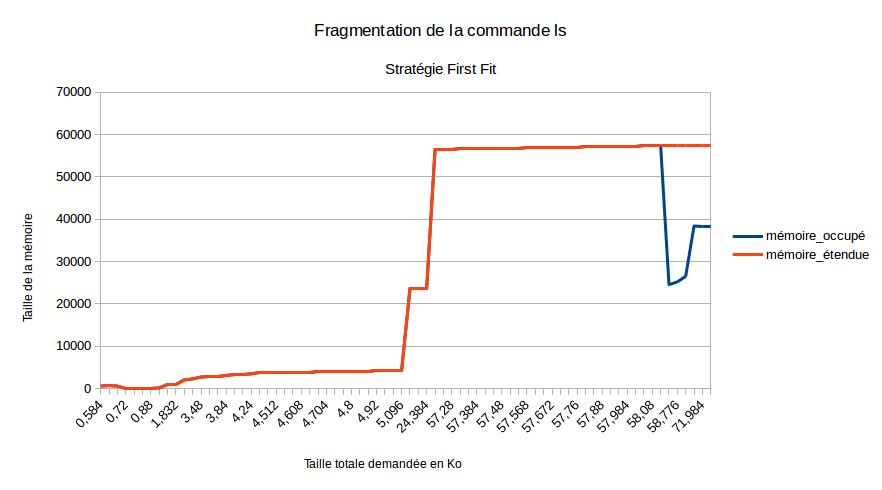
\includegraphics[width=15cm]{ls_firstfit.jpg}
\end{center}
	\item gcc

\begin{center}	
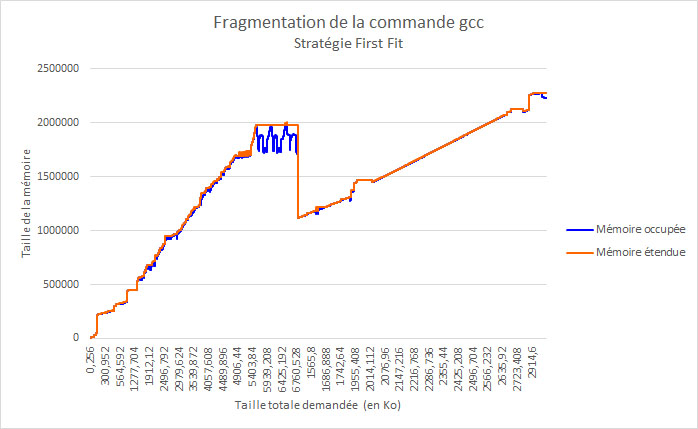
\includegraphics[width=12cm]{gcc_firstfit.jpg}
\end{center}
\end{itemize}

\subsection{Avec la stratégie Best Fit}
\begin{itemize}
	\item ls
	
\begin{center}	
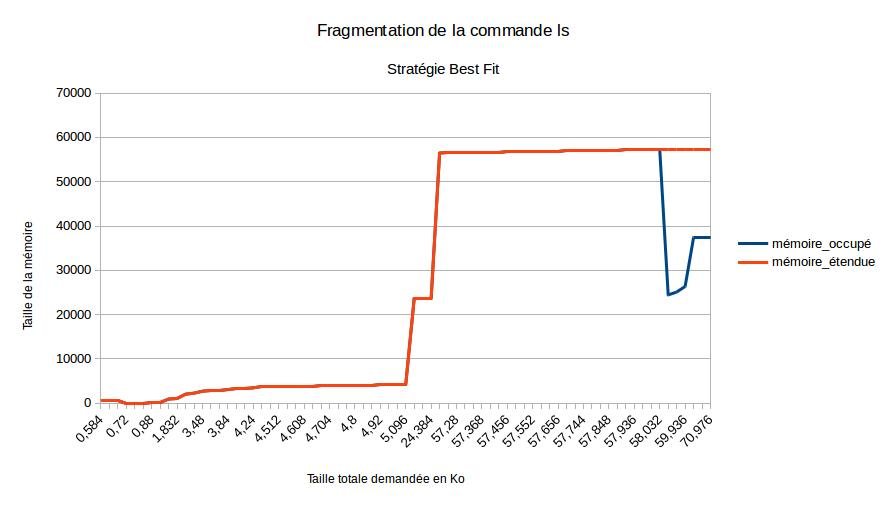
\includegraphics[width=15cm]{ls_bestfit.jpg}
\end{center}
	\item gcc

\begin{center}	
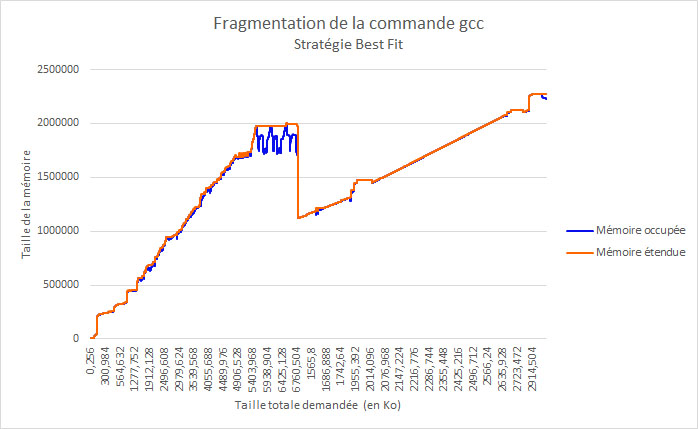
\includegraphics[width=12cm]{gcc_bestfit.jpg}
\end{center}
\end{itemize}

\subsection{Avec la stratégie Worst Fit}
\begin{itemize}
	\item ls

\begin{center}	
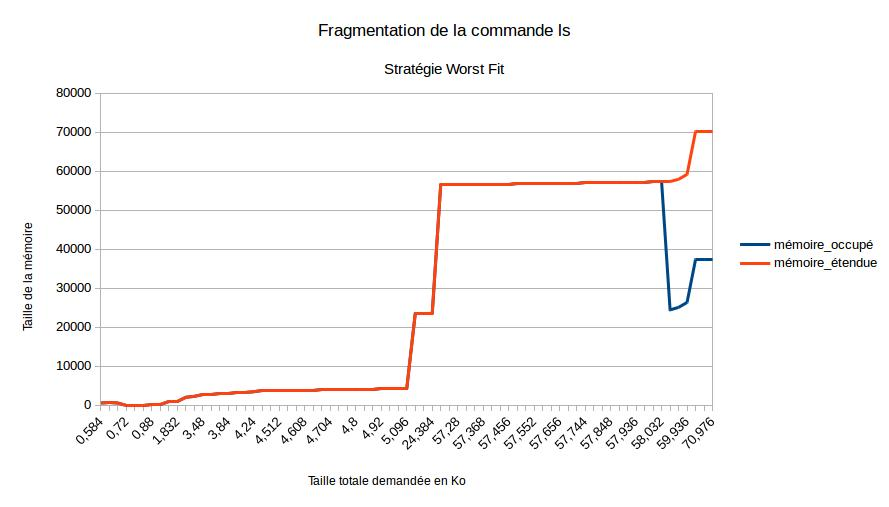
\includegraphics[width=15cm]{ls_worstfit.jpg}
\end{center}
	\item gcc
	
\begin{center}	
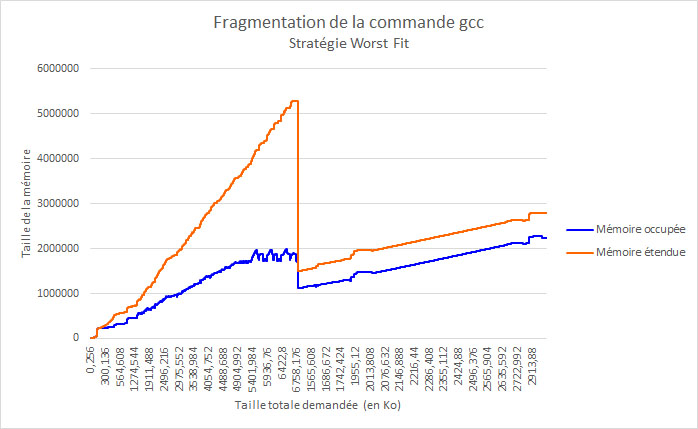
\includegraphics[width=12cm]{gcc_worstfit.jpg}
\end{center}
\end{itemize} 
 
\section{Conclusion}

\end{document}